\section{Settings}
In this section, we start by presenting the departure time choices problem for individual users. Then we proceed by characterizing the optimal departure time under different scheduling preferences and exogenous travel time profiles.


\subsection{Arrival times and travel costs}
\label{sec:cost_fn}

\label{sec:theory}

Consider some users commuting between an origin and a destination. The travel time between the origin-destination (OD) pair fluctuates across the time of the day. To hedge against time-varying congestion, some users may be motivated to arrive early and later at their destinations to avoid the rush hours.



To capture such trade-offs, we follow the bottleneck model by considering that each user chooses an arrival time $t_a$ at their destination that minimizes their individual travel cost  \footnote{When $tt_a'(t_a) < 1$ for all $t \in \mathcal{T}$, it is consistent with the departure time choice problem in \cite{arnott1993structural}. The reason is that there will be a one-to-one correspondence between any arrival time $t_a$ and the departure time $t_d = t_a - tt_a(t_a)$ because $\partial t_d/\partial t_a > 0$ in this case. }. Let $\mathcal{T}$ be the set of all possible arrival times. The travel cost by arriving at any time $t_a 
 \in \mathcal{T}$ is defined as 
\begin{equation}
  \label{eq:cost_ta}
  C(t_a) = \alpha tt_a(t_a) + \beta[t^*-t_a]^+ + \gamma[t_a-t^*]^+,
\end{equation}
where $tt_a(t_a)$ denotes the experienced travel time for travelers arriving at time $t_a$, \(t^*\) is the desired arrival time at the destination,  \(\alpha\) is the value of travel time, and \(\beta\) and \(\gamma\) are respectively the unit costs of arriving early and late at the destination. Without loss of generality, from now on, we normalize the value of $\alpha$ to 1.


 An implied assumption here is that all travelers arriving at the same destination would always experience the same travel time, which enables the definition of $tt_a(t_a)$. The travel time profile is assumed to be exogenous, which is not affected by an individual traveler's choices.  In addition, we start with a representative congestion pattern such that the travel time profile function is subject to the following assumption. 

\begin{assumption}\label{ass:continous}
   The travel time profile function $tt_a(t_a)$ is continuous, nonnegative, and bounded. 
\end{assumption}

\subsection{Minimum of the cost function}
\label{sec:cost_minima}

Next, we characterize the arrival time preference for an individual user with given scheduling preferences parameterized by $\beta, \gamma$, and $t^*$. Recall that users choose their arrival times to minimize their individual travel cost, and we define the minimal travel cost $C^{opt}$ as
    \begin{equation*}
      C^{opt} = \min_{t_a \in \mathcal{T}}C(t_a).
    \end{equation*} 

To facilitate our discussion, we introduce two technical terms regarding the conditional minima of the travel cost function $C(t_a)$: the minimal early arrival cost$$C_e^{opt}  = \min_{t_a \le  t^*}C(t_a)$$ and the minimal late arrival cost  $$C_l^{opt} =  \min_{t_a \ge  t^*}C(t_a).$$ 

\begin{definition}\label{def:CEA}
    Given any travel time profile function $tt_a(t_a)$ and \(\beta\),  an interval $[t_e, \bar t_e]$ with $\bar t_e > t_e$ is termed an early arrival (EA) interval when the following condition holds:
\begin{equation}\label{eq:increase_faster}
    tt_a(t ) \ge tt_a(t_e)  + \beta (t - t_e ), \forall t \in [t_e, \bar t_e].
\end{equation} 
\end{definition}

\begin{definition}
    Given any travel time profile function $tt_a(t_a)$ and \( \gamma\), an interval $[\bar t_l, t_l]$ with $t_l >\bar t_l$ is termed a late arrival (LA) interval when the following conditions hold:
    \begin{equation}\label{eq:decrease_faster}
        tt_a(t_l)  + \gamma  (t - t_l ) \ge  tt_a(t ), \forall  t \in [\bar  t_l, t_l].
\end{equation} 
 
\end{definition}

Roughly speaking, congestion increases (respectively, decreases) rapidly with the arrival time within each EA (LA) interval, such that the time savings from arriving earlier (later) outweigh the cost of early arrival. 

\begin{definition}
 An EA (respectively, LA) interval is said to be a critical EA (CEA) or critical LA (CLA) interval if it is not strictly contained within any other EA (LA) interval.
\end{definition}

The following graph illustrates the CEA and CLA intervals in a general travel time profile function $tt_a$. As we can observe, there are two CEA intervals and two CLA intervals. The first CEA interval overlaps with the first CLA interval, while the second CEA and CLA intervals are disjoint.
 

\begin{figure}
  \centering
  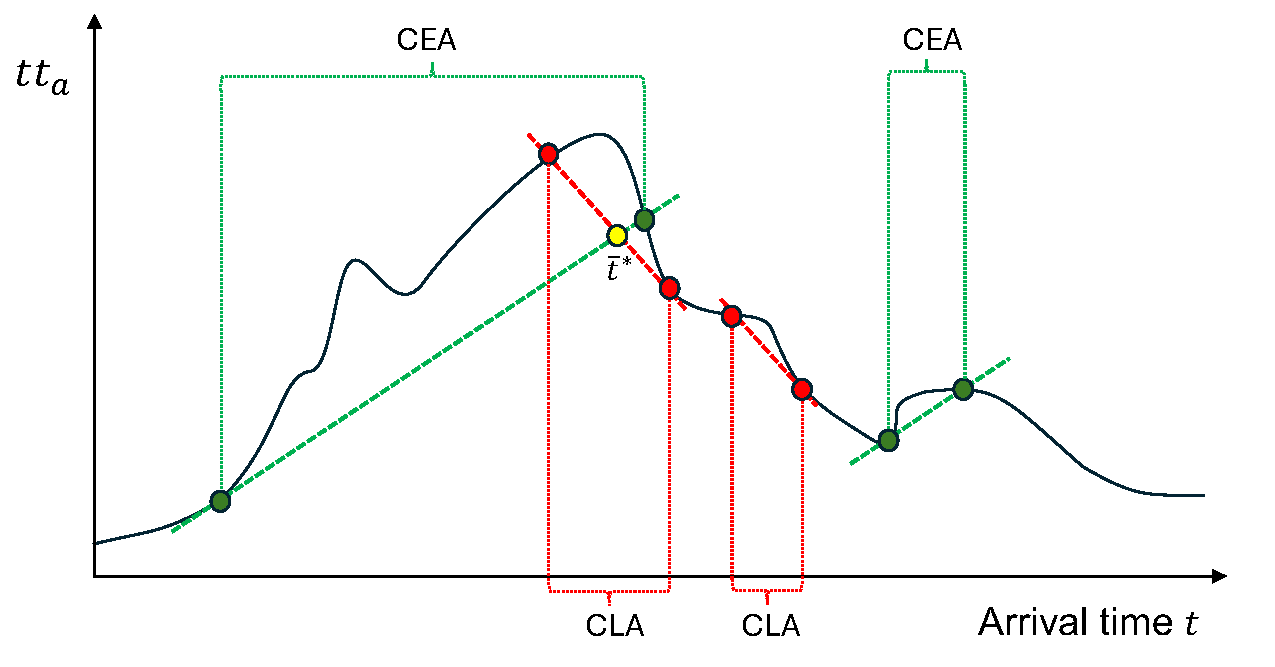
\includegraphics[width=.8\textwidth]{illustration.pdf}
  \caption{An example of the CEA and CLA intervals for a general travel time profile function}
  \label{fig:illustration}
\end{figure}


% \begin{lemma}
%     Each EA interval corresponds to exactly one critical CEA interval.
% \end{lemma}

\begin{lemma}\label{lemma:disjoint}
Any two critical early arrival (CEA) intervals or two critical late arrival (CLA) intervals are disjoint.
\end{lemma}

\begin{proof}
Suppose that there are two CEA intervals $[t_e, \bar t_e]$ and $[t_e', t_l']$ overlapping with each other, i.e., $t_e' \le t_l$ and $t_e \le t_l'$. Then for any $t$ in the overlapped part $[t_e', t_l]$, the condition still holds: 
$$
tt_a(t ) \ge tt_a(t_e)  + \beta (t - t_e ).
$$
Thus, the interval $[t_e, t_l']$ is an EA interval and it contains  $[t_e, t_l]$ and $[t_e', t_l']$. This contradicts the definition of CEA intervals. The proof for CLA intervals is similar and therefore omitted here. 
\end{proof}

By Lemma \ref{lemma:disjoint}, each desired arrival time $t^*$ can fall into at most one CEA (CLA) interval, which leads to the following proposition. 

\begin{prop}
  \label{prop:into-early}
 Under Assumption \ref{ass:continous}, given any $tt_a(t)$, $\beta$, and $t^*$, the minimal early arrival cost is  
$$C_e^{opt} = \begin{cases}
    C(t_e),  \text{if }\exists [t_e, \bar{t}_e] \in E \text{ such that } t^* \in [t_e, \bar{t}_e],\\
     tt_a(t^*), \text{otherwise}. 
\end{cases}$$
where $E$ denotes the set of all critical early arrival (CEA) intervals.
\end{prop}


% \begin{prop}
%   \label{prop:into-early}
% Under Assumption \ref{ass:continous}, if there exists a critical early arrival (CEA) interval $[t_e, \bar{t}_e]$ for a given early arrival penalty $\beta$, then (1) the minimal early arrival cost for any desired arrival time $t^* \in [t_e, \bar{t}_e]$ is attained at $t_e$, i.e., 
% $C_e^{opt} = C(t_e)$. 
% \end{prop}
\begin{proof}
Recall that the minimal early arrival cost  $C_e^{opt}$ is defined as $$C_e^{opt} = \min_{t \le t^*} C(t).$$

(1) We start by discussing the case when there exists some CEA interval $[t_e, \bar{t}_e]$ such that  $t^* \in [t_e, \bar{t}_e]$.  To show that $C_e^{opt}$ is achieved at $t_e$, it is equivalent to show that $C(t) \ge C(t_e) $ for any $t \le t^*$. We proceed to show that $C(t) \ge C(t_e)$ in two cases when $t \in [t_e, t^*]$ and $t < t_e$, respectively.    

Case 1: $t \in [t_e, t^*]$.  Recall that the trip cost at any $t \in [t_e, t^*]$ can be written as 
$$C(t) = tt_a(t) + \beta (t^* - t).$$
Using Inequality \eqref{eq:increase_faster} from Definition \ref{def:CEA} of CEA intervals, i.e., $$tt_a(t ) \ge tt_a(t_e)  + \beta (t - t_e ), \forall t \in [t_e, \bar t_e],$$ we obtain that 
$$C(t) \ge tt_a(t_e) + \beta (t - t_e ) + \beta (t^* - t) = C(t_e), \forall t \in [t_e, \bar t_e].$$
Thus, we have $C(t) \ge C(t_e) $ for any $t \in [t_e, t^*]$.

Case 2: $t < t_e$. We prove that $C(t) \ge C(t_e) $ for any $t < t_e$ by contradiction. Suppose that there exists some $t'< t_e$ such that $C(t') < C(t_e)$.  Define a set 
\begin{equation}\label{eq:def_T}
    T = \{t \in [t', t_e] \mid tt_a(t')  + \beta (t - t' ) =  tt_a(t )\},
\end{equation}
and let $t'' = \max(T).$ Apparently, $C(t) = C(t')$ for any $t \in T$. Next, we will prove that the interval $[t'', \bar{t}_e]$ is a CEA interval, which contains $[t_e, \bar{t}_e]$, contradicting the definition of a critical early arrival interval.


To do so, we prove that the following condition holds by Definition \ref{def:CEA}:
$$ tt_a(t'')  + \beta (t - t'' ) \le  tt_a(t ), \forall t \in [t'', \bar t_e].$$ 

First, we show that $ tt_a(t'')  + \beta (t - t'' ) \le  tt_a(t )$ holds for any $ t \in [t_e, \bar t_e] $. Recall that $[t_e, \bar t_e]$ is a CEA interval, and therefore by definition the following inequality holds:
$$tt_a(t_e)  + \beta (t - t_e ) \le  tt_a(t ), \forall t \in [t_e, \bar t_e].$$ 
Given that $C(t') < C(t_e)$ by assumption and $C(t'') = C(t')$ by definition, we have $C(t'') < C(t_e)$.  Thus, we have $$tt_a(t'')  + \beta (t - t'' ) < tt_a(t_e)  + \beta (t - t_e ), \forall t \in [t_e, \bar t_e]. $$
That is, $$tt_a(t'')  + \beta (t - t'' ) <  tt_a(t ), \forall t \in [t_e, \bar t_e].$$

Second,  we show that $ tt_a(t'')  + \beta (t - t'' ) \le  tt_a(t )$ holds for any $ t \in [t'',  t_e]$.  Let $ f(t)= tt_a(t)  + \beta (t'' - t ) -  tt_a(t'' ) $, which is continuous.  We have shown above that $$tt_a(t'')  + \beta (t_e - t'' ) <  tt_a(t_e),$$
i.e., $f(t_e) <0$. Also, we have $f(t'') =0$ by definition. 

Suppose that there exists some $t \in (t'',  t_e)$ such that $$tt_a(t)  + \beta (t'' - t ) >  tt_a(t'' ),$$ i.e., $f(t) <0$. By the continuity of $f(t)$, there must be some $t''' \in (t, t_e)$ such that $f(t''')=0,$ i.e., $$tt_a(t''')  + \beta (t'' - t''' ) =  tt_a(t'' ).$$
Therefore, we have $t''' \in T$ and $t''' > t''$, which contradicts the condition that $t'' =\max(T)$. Thus, we must have $ tt_a(t'')  + \beta (t - t'' ) \le  tt_a(t )$ holds for any $ t \in [t'',  t_e]$. 

(2) Now we turn to discuss the case when $t^*$ does not fall into any CEA intervals. Again, we prove by contradiction. Suppose that there exists some $t' < t^*$ such that $C(t') < C(t^*)$. Redefine a set 
\begin{equation}\label{eq:def_T_2}
    T = \{t \in [t', t^*] \mid tt_a(t')  + \beta (t - t' ) =  tt_a(t )\}, 
\end{equation} 
and still let $t'' = \max(T)$. Since $C(t') < C(t^*)$, we have 
$$tt_a(t') + \beta (t^* - t') < tt_a(t^*).$$
Using that $tt_a(t'')  + \beta (t - t'' )  = tt_a(t')  + \beta (t - t' )  = tt_a(tt') $, we have 
$$tt_a(t'') + \beta (t^* - t'') < tt_a(t^*).$$
Also, the following equation naturally holds: 
$$tt_a(t'') + \beta (t'' - t'') = tt_a(t'').$$
By continuity and contradiction,  we are able to show that $$tt_a(t'') + \beta (t - t'') \le tt_a(t), \forall t \in [t'', t^*].$$
That is, $[t'', t^*] $ is an EA interval. And there always exists some CEA interval that contains $[t'', t^*]$. Therefore, $t^*$ would fall into some CEA interval, which contradicts.  The proof is completed.  


\end{proof}

In parallel, we can prove the following proposition concerning late arrivals. The proof is similar to the proof for Proposition \ref{prop:into-early} and therefore omitted here. 


\begin{prop}
  \label{prop:into-late}
 Under Assumption \ref{ass:continous}, given any $tt_a(t)$, $\gamma$, and $t^*$, the minimal late arrival cost is  
$$C_l^{opt} = \begin{cases}
    C(t_l),  \text{if }\exists [\bar{t}_l, t_l] \in L \text{ such that } t^* \in [\bar{t}_l, t_l],\\
     tt_a(t^*), \text{otherwise}. 
\end{cases}$$
where $L$ denotes the set of all critical late arrival (CLA) intervals.
\end{prop}


 Propositions \ref{prop:into-early} and \ref{prop:into-late} are used to identify the minimal travel cost $C^{opt}$ by comparing the MEAC $C_e^{opt}$ and the MLAC $C_l^{opt}$. There are four cases to be discussed, of which the first three cases can be directly derived with Propositions \ref{prop:into-early} and \ref{prop:into-late}. 

\begin{corollary}
     Under Assumption \ref{ass:continous},  if the desired arrival time $t^*$ does not fall into any CEA or CLA intervals, then the minimal travel cost is $C^{opt} = tt_a(t^*)$. 
\end{corollary}
\begin{proof}
    We have $C_e^{opt} = tt_a(t^*)$ by Proposition \ref{prop:into-early} and $C_l^{opt} = tt_a(t^*)$ by Proposition \ref{prop:into-late}. Therefore, the corresponding minimal travel cost is $C^{opt} = tt_a(t^*)$. Namely, it is optimal to arrive on time. 
\end{proof}

 \begin{itemize}
     \item Case 1: the desired arrival time $t^*$ does not fall into any CEA or CLA intervals. We have $C_e^{opt} = tt_a(t^*)$ by Proposition \ref{prop:into-early} and $C_l^{opt} = tt_a(t^*)$ by Proposition \ref{prop:into-late}. Therefore, the corresponding minimal travel cost is $C^{opt} = tt_a(t^*)$. Namely, it is optimal to arrive on time. 
 
  \item  Case 2: the desired arrival time  $t^*$ falls into a CEA interval but not any CLA interval. We have $C_e^{opt} \le tt_a(t^*)$ by Proposition \ref{prop:into-early} while $C_l^{opt} = tt_a(t^*)$ by Proposition \ref{prop:into-late}.  Then we can immediately conclude that $C_e^{opt} \le C_l^{opt}$ and therefore the corresponding minimal travel cost is $C^{opt} = C_e^{opt}$. Namely, it is optimal to arrive early.  
 
  \item  Case 3: the desired arrival time $t^*$ falls into a CLA interval but not any CEA interval. Similarly, the corresponding minimal travel cost is $C^{opt} = C_l^{opt}$. Namely, it is optimal to arrive late. 
 \end{itemize}
 
In Case 4, the desired arrival time $t^*$ falls into both a CEA interval and a CLA interval. The discussion is formalized in the following proposition. 

\begin{prop}
Suppose that there exists a CEA interval $[t_e, \bar t_e]$ and a CLA interval $[\bar t_l,  t_l]$ such that $t^* \in [t_e, \bar t_e]$ and $t^* \in [\bar t_l,  t_l]$.  Under Assumptions \ref{ass:continous}, there exists a desired arrival time threshold $$\bar t^* = \frac{tt_a(t_l) - tt_a(t_e) + \beta t_e + \gamma t_l}{\beta + \gamma}$$
   such that 
$$\begin{cases}
   C_e^{opt} < C_l^{opt} ,  \text{if } t^* < \bar t^*, \\
      C_e^{opt} = C_l^{opt}, \text{if }  t^* = \bar t^*, \\
   C_e^{opt} > C_l^{opt},  \text{if }  t^* > \bar t^*.
\end{cases}$$


\end{prop}

\begin{proof}
Note that at the threshold $\bar t^*$, by definition we have $$tt_a(t_e) + \beta(\bar t^* - t_e) = tt_a(t_l) + \gamma(t_l- \bar t^*).$$
Since $[t_e, \bar t_e]$ is a CEA interval, and $[\bar t_l,  t_l]$ is a CLA interval, by Propositions \ref{prop:into-early} and \ref{prop:into-late}, we have $$C_e^{opt} = C(t_e) = tt_a(t_e) + \beta(t^* - t_e), $$ $$C_l^{opt} = C(t_l) = tt_a(t_l) + \gamma( t_l-t^*).$$
Thus, we have $C_e^{opt} = C_l^{opt} $ when $t^* = \bar t^*$. Obviously, we have $\partial C_e^{opt}/\partial t^* >0$ and $\partial C_l^{opt}/\partial t^* <0$, which leads to that $\partial (C_e^{opt} -  C_l^{opt}) /\partial t^* <0 $. The proof is completed. 
\end{proof}

Note that the threshold $\bar t^*$ is not necessarily in the CEA interval or the CLA interval when one of the intervals contains the other.  

\subsection{A representative case}

Now, we continue the analysis based on a typical congestion pattern, subject to the following assumption.
\begin{assumption}\label{ass:twiceDiff}
   The travel time profile function $tt_a(t)$ is unimodal and twice differentiable. There exists an interval $   \mathcal{D}_{conc} = [k_1, k_1]$ such that $tt_a(t)$ is concave in $\mathcal{D}_{conc}$, and convex otherwise. 
\end{assumption}

Roughly speaking, under Assumption \ref{ass:twiceDiff}, congestion will monotonically increase during the day up until a certain threshold time, and then monotonically decrease afterwards. Additionally, it requires the derivative of the travel time to be unimodal both before and after the peak.



\begin{prop}
Under Assumptions \ref{ass:continous} - \ref{ass:twiceDiff}, there exist at most one CEA interval $[t_e, \bar t_e]$ and at most one CLA interval $[\bar t_l, t_l]$ such that $tt_a'(t_e)= \beta$ and $ tt_a'(t_l)= \gamma$.
\end{prop}
\begin{proof}
By Proposition \ref{prop:into-early}, the left endpoint of a CEA interval is a minimum of the cost function, i.e., $C(t_e) = \min_{t \le t^*} C(t)$ with 
   $$C(t) = tt_a(t) + \beta (t^* - t).$$
Under Assumption \ref{ass:twiceDiff}, the function $tt_a$ is twice differentiable. Thus, by the optimality condition, we have 
\begin{align}
tt_a'(t_i^e) = \beta,\\
tt_a''(t_i^e) \geq 0.
\end{align}

By Assumption \ref{ass:twiceDiff}, when $t < k_1$, $tt_a(t)$ is convex and increasing in $t$. Then $tt'_a(t)$ is monotonically increasing in $t$ when $t< k_1$. Thus, there is at most one $t < k_1$ such that $tt_a'(t) = \beta$. When $t \in [k_1, k_2]$,  $tt_a(t)$ is concave and therefore $tt_a''(t) \le 0$. When $t >k_2$,  $tt_a(t)$ is concave and decreasing in $t$, i.e., $tt_a'(t)\le 0$ for all $t > k_2$.  Therefore, there is at most one $t \in \mathcal{T}$ such that $tt_a'(t) = \beta$ and $tt_a''(t) \geq 0$. Namely, there is at most one CEA interval. Similarly, we can show that there is at most one CLA interval. The proof is completed. 
\end{proof}



Further, we consider that the congestion pattern, described by the travel time profile, is such that a traveler will not arrive earlier than anyone who departs earlier than her/him, which is termed as the first-in-first-out (FIFO) rule in literature. Thus, we impose the following assumption regarding the travel time function  $tt_a(t_a)$.



\begin{assumption}\label{ass:FIFO}
The travel time profile function $tt_a(t_a)$ is differentiable, and $tt'_a(t_a) \le 1$. 
\end{assumption}


Under Assumption \ref{ass:FIFO}, the FIFO principle is always satisfied. To see this, it is equivalent to show that the arrival time $t_a$ is weakly increasing in the departure time $t_d$, i.e., $\partial t_d / \partial t_a \ge 0$ under Assumption \ref{ass:FIFO}.  Note that by definition, we have $ t_d = t_a - tt_a(t_a)$.  Obviously, when $tt'_a(t_a) \le 1$, we have $\partial t_d / \partial t_a = 1 - tt_a'(t_a) \ge 0$. Therefore, a traveler will arrive earlier if she departs earlier. 



$C(t_a)$, i.e.,  $t_a^* = \text{arg} \min C(t_a)$. The individual travel cost $C(t_a)$ is defined as 

we consider a cost function of the form

\begin{equation}
  \label{eq:cost-t_d}
  C(t_d; \alpha, \beta, \gamma, t^*) = \alpha tt(t_d) + \beta[t^*-t_d-tt(t_d)]^+ + \gamma[t_d+tt(t_d)-t^*]^+ 
\end{equation}
where
\begin{itemize}
\item \(t_d\) is a possible departure time, on which the cost depends
\item \(t^*\) is the desired arrival time
\item \(\alpha\) is the value of time spent travelling
\item \(\beta\) is the value of time spent waiting there
\item \(\gamma\) is the value of time arriving late
\item \(tt(t_d)\) is the time spent traveling if leaving at time \(t_d\)
\item \([x]^+ = \max(0, x)\)
\end{itemize}

We will consider, in this article,
how the cost depends on the time at which a person arrives,
rather than the time at which the person departs.
Since the travel time is known without uncertainty,
the users will then be able to make a choice based on their arrival time.

Let thus
\begin{equation}
  \label{eq:t_a-t_d}
  t_a(t_d) = t_d + tt(t_d)
\end{equation}
be the function linking the departure time to the arrival time.
The following holds:
\begin{obs}
  \label{obs:inv-t_a}
  The function \(t_a(t_d)\) is invertible
\end{obs}
This simply follows from noting that  \(t_a(t_d)\) must be strictly increasing:
this corresponds to the traffic following a First In First Out (FIFO) logic,
that is, a later departure cannot result in an earlier arrival:
a reasonable assumption that we make on the travel time function.

The function \(t_d(t_a)\) that, given an arrival time,
yields the unique departure time that would result in the given arrival,
is thus well defined.
The travel time function can hence be defined in term of the arrival time:
\begin{definition}
  \label{def:tta}
  Let
  \begin{equation*}
    tt:\R \rightarrow \R
  \end{equation*}
  be a function expressing the travel time in terms of the departure time.
  The function \(tt_a\), expressing the travel time in terms of the arrival time, is defined as follows:
  \begin{equation*}
    tt_a(t_a) = tt(t_d(t_a))
  \end{equation*}
\end{definition}

The assumption of the traffic following a FIFO logic has different implications,
on the functions \(tt\) and \(tt_a\):

\begin{lemma}
  \label{lemma:bounded-der-tt}
  Suppose the travel time functions \(tt, tt_a\) to be differentiable.
  
  The traffic follows a First In First Out logic if and only if the function \(tt\) satisfies
  \begin{equation*}
    tt'(t_d) > -1\quad \forall \, t_d
  \end{equation*}
  or, equivalently, the function on arrival time \(tt_a\) satisfies
  \begin{equation*}
    tt_a'(t_a) < 1\quad \forall \, t_a
  \end{equation*}
\end{lemma}
\begin{proof}
  Note that the traffic follows a FIFO logic if and only if the function \(t_a(t_d)\) is strictly increasing,\todo{split sentence}
  and, once defined, its inverse \(t_d(t_a)\) will be so.
  
  Being \(t_a(t_d)\) differentiable, it is strictly increasing if and only if its derivative is positive:
  \begin{align*}
    \diffp{}{{t_d}} t_a(t_d) & > 0 \\
    1 + tt'(t_d) & > 0 \\
    tt'(t_d) & > -1
  \end{align*}
  
  Alternatively, consider its inverse
  \begin{equation*}
    t_d(t_a) = t_a - tt_a(t_a)
  \end{equation*}

  Again, it is increasing if and only if it has positive derivative:
  \begin{align*}
    \diffp{}{{t_a}} t_d(t_a) & > 0 \\
    1 - tt_a'(t_a) & > 0 \\
    tt_a'(t_a) < 1
  \end{align*}
\end{proof}

Once this needed property on the travel time function was stated,
the cost function can be simplified by expressing it in function of the arrival time:
by using equation \eqref{eq:t_a-t_d} and Definition~\ref{def:tta},
the expression for the cost in~\eqref{eq:cost-t_d} indeed simplifies,
becoming

\begin{equation}
  \label{eq:cost-t_a}
  C(t_a; \alpha, \beta, \gamma, t^*) = \alpha tt_a(t_a) + \beta[t^*- t_a]^+ + \gamma[t_a - t^*]^+ 
\end{equation}
where the dependency of \(t_a\) on the departure time \(t_d\) has been hidden:
the arrival time can indeed be directly observed,
and its dependency on the departure time neglected.

In the following article,
the expression used will be the one given the arrival time, as shown in~\eqref{eq:cost-t_a},
being that a simpler expression if compared to the original one in~\eqref{eq:cost-t_d}.

We will, lastly normalize \(\alpha\) to 1.
This is possible since the cost can be considered up to a multiplicative constant.
Instead of the real cost \(C\) we will thus consider a scaled version of it \(C/\alpha\),
and minimize the following:
\begin{equation}
  \label{eq:cost_final}
  C(t_a; \beta, \gamma, t^*) = tt_a(t_a) + \beta[t^*- t_a]^+ + \gamma[t_a - t^*]^+ 
\end{equation}

The notation is here ambiguous regarding the cost \(C\) and the coefficients \(\beta,\gamma\).
It anyway doesn't lose in generality, and was chosen for simplicity.

\subsection{Minimum of the Cost Function}
\label{sec:cost_minima}



Consider hence the cost in \eqref{eq:cost_final},
and the problem of finding the minimum of it.
Before computing the first order condition,
in order to find the global minimum it is useful to do some qualitative reasoning on the values taken by the cost function.

Note that, indeed, a value \(t_0\) for the arrival time can only be greater,
smaller or equal to the given \(t^*\).
In the following definition,
the two cases are separated, so that they can be studied independently.
\begin{definition}
  Let values for the parameters \(\beta, \gamma, t^*\) be fixed.
  \begin{itemize}
  \item The \textbf{optimal early arrival} \(t_e^{opt}\) is the early arrival realizing the least cost:
    \begin{equation*}
      t_e^{opt}(\beta, \gamma ,t^*) = \argmin_{t_a < t^*}C(t_a; \beta, \gamma, t^*)
    \end{equation*}
  \item The \textbf{optimal late arrival} \(t_l^{opt}\) is the late arrival realizing the least cost:
    \begin{equation*}
      t_l^{opt}(\beta, \gamma ,t^*) = \argmin_{t_a > t^*}C(t_a; \beta, \gamma, t^*)
    \end{equation*}
  \item The \textbf{optimal arrival} \(t^{opt}\) is the arrival realizing the least cost:
    \begin{equation*}
      t^{opt}(\beta, \gamma ,t^*) = \argmin_{t_a}C(t_a; \beta, \gamma, t^*)
    \end{equation*}\todo{Set tie breaking rule}
  \end{itemize}
\end{definition}

Please note that in general,
optimal early and late arrivals may not exist,
depending on the choice of the travel time function and the parameters.
The zones in which these minima exist will be studied later.

For studying where these minima occur, consider now the case of an early arrival \(t_a = t_0 < t^*\).
Since
\begin{equation*}
  t_0 - t^* < 0
\end{equation*}
the cost simplifies, becoming
\begin{align}
  C(t_0; \beta, \gamma, t^*) & = tt_a(t_0) + \beta[t^*- t_0]^+ + \gamma[t_0 - t^*]^+ \nonumber \\
                             & = tt_a(t_0) + \beta(t^*- t_0)\label{eq:cost_early}
\end{align}

\begin{figure}
  \centering
  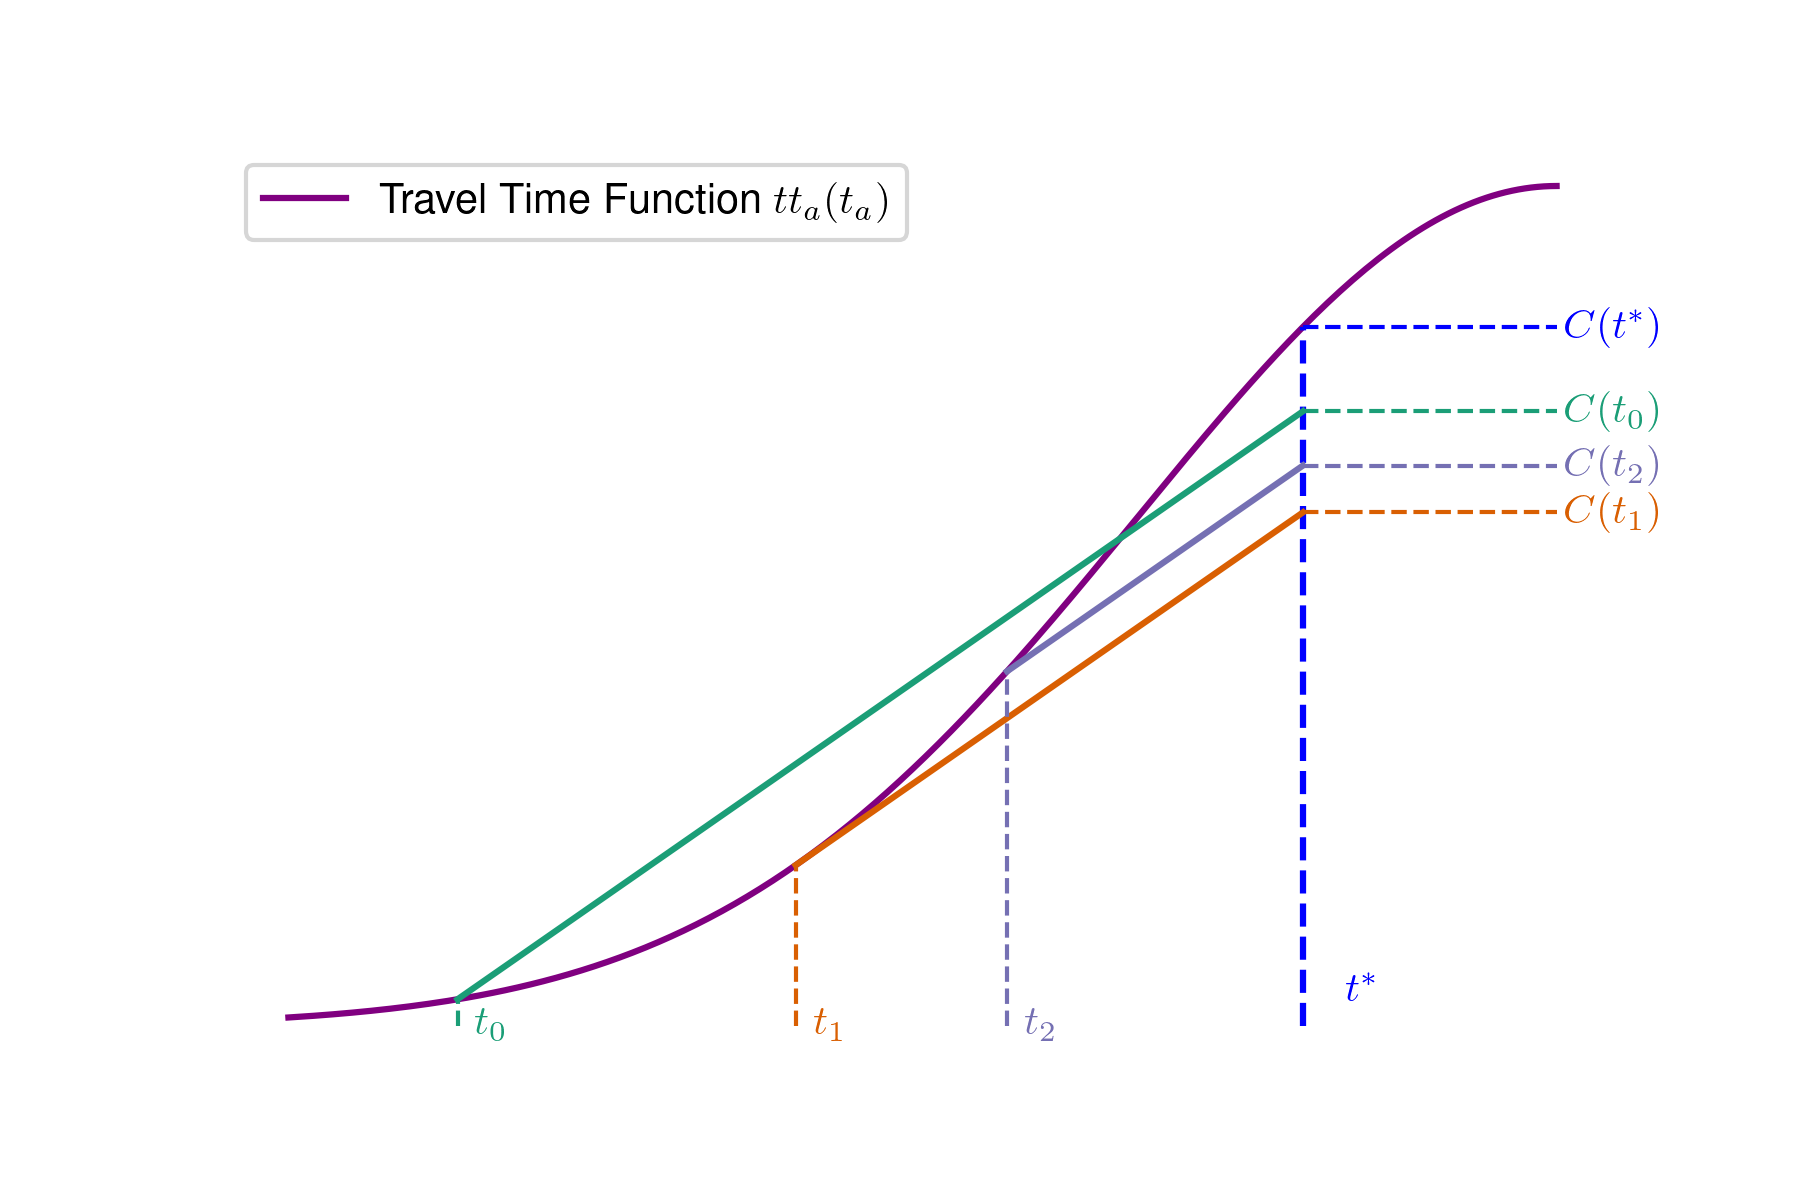
\includegraphics[width=.8\textwidth]{early_arrivals_cost}
  \caption{Dependency of the cost on the arrival time, for early arrival.
    The solid lines are parallel, of slope \(\beta\).
  Note that their distance is the only factor affecting the cost of an early arrival}
  \label{fig:early_arrivals_cost}
\end{figure}

The cost will thus be, as expected,
the sum of the travel time and a term linear on the distance of the actual arrival from the desired one.

Figure \ref{fig:early_arrivals_cost} displays how the cost of an early arrival changes when varying the arrival time:
the cost is only determined by the distance of the lines of slope \(\beta\) between each other, that is,
the projected distance of the points \(tt_a(t_a)\) on the axis orthogonal to the lines determining the cost
(the one described by \(y = -x/\beta\)).

This reasoning leads to the following lemma:
\begin{lemma}
  \label{lemma:cost_decoupled}
  If an optimal early arrival \(t_e^{opt}\) exists,
  it can be found by solving a simple minimization problem:
  \begin{equation*}
    t_e^{opt} = \argmin_{t_a < t^*} (tt_a(t_a) - \beta t_a)
  \end{equation*}

  Similarly, if an optimal late arrival exists,
  it is
  \begin{equation*}
    t_l^{opt} = \argmin_{t_a > t^*} (tt_a(t_a) + \gamma t_a)
  \end{equation*}
\end{lemma}
\begin{proof}
  The claim for early arrivals simply follows from the expression for the cost in~\eqref{eq:cost_early}:
  the following indeed holds for \(t_a < t^*\)
  \begin{align*}
    C(t_a; \beta, \gamma, t^*) & = tt_a(t_a) + \beta(t^*- t_a) \\
                               & = tt_a(t_a) + \beta t^* - \beta t_a
  \end{align*}

  But \(\beta t^*\) is clearly constant in \(t_a\),
  and minimization is invariant on translations.
  This yields
  \begin{align*}
    t_e^{opt} & = \argmin_{t_a < t^*} C(t_a) \\
              & = \argmin_{t_a < t^*} (tt_a(t_a) + \beta t^* - \beta t_a) \\
              & = \argmin_{t_a < t^*} (tt_a(t_a) - \beta t_a)
  \end{align*}

  Regarding late arrivals, the argument is symmetrical and thus omitted.
\end{proof}

Note that this has some trivial implication on the value of the derivative of the travel time function at the optimal points:
\begin{obs}
  \label{obs:foc}
  The derivative of the travel time function \(tt_a'\) is fixed at the optimal points:
  \begin{itemize}
  \item \(tt_a'(t_e^{opt}) = \beta\)
  \item \(tt_a'(t_l^{opt}) = -\gamma\)
  \end{itemize}
\end{obs}

This follows from the Lemma above:
if the function \(tt_a\) is differentiable, being the minima computed over an open set,
if they exist they necessarily satisfy the first order conditions.
The function \(tt_a(t_a) - \beta t_a\) is minimized for
\begin{equation*}
  tt_a'(t_a) = \beta
\end{equation*}
The case for late arrival is analogous.\todo{similarly, for late arrivals we get...}

While not particularly difficult to retrieve,
the expression in Lemma~\ref{lemma:cost_decoupled} is useful,
since it makes a clearer decoupling of the dependencies of the point that minimizes the cost on the parameters \(\beta, \gamma\) and \(t^*\).
We can indeed see how changing the parameters affects the location of the points \(t_e^{opt}, t_l^{opt}\).
This is described by the following proposition:
\begin{prop}
  \label{prop:into-early-late}
  \textcolor{red}{We need continuity, bounded}
  Given a value for the parameters \(\beta, \gamma\),
  there exist two collections of disjoint intervals
  \begin{align*}
    E & = \{(t_e^i, \bar{t_e^i})\}_i,\quad i = 1, \dots, n \\
    L & = \{(\bar{t_l^j}, t_l^j)\}_j,\quad j = 1, \dots, m \\
  \end{align*}
  such that, if exists a value for \(i\) such that \(t^* \in (t_e^i, \bar{t_e^i})\),
  the optimal early arrival will be the lower bound of the interval:
  \begin{equation*}
    t_e^{opt}(\beta, \gamma, t^*) = t_e^{i}
  \end{equation*}

  Similarly, if exists a value for \(j\) such that \(t^* \in (\bar{t_l^j}, t_l^j)\),
  the optimal late arrival will be the upper bound of the interval:
  \begin{equation*}
    t_l^{opt}(\beta, \gamma, t^*) = t_l^{j}
  \end{equation*}

  If such a value for \(i\) (or \(j\)) does not exist,
  then the optimal early (respectively, late) arrival is not defined.
\end{prop}

\begin{proof}
  If there is no \(t^*\) for which an optimal early arrival is defined,
  then setting \(n = 0\) trivially proves the proposition.

  Suppose now that there exist a desired arrival time \(t_0\) such that \(t_e^{opt}(\beta, \gamma, t_0)\) is defined.

  Since we are assuming \(tt_a\) to be continuous\todo{Where is this assumption stated?},
  the cost will be continuous as well,
  and early arrivals can approximate arbitrarily well the cost of an on-time arrival:
  \begin{equation*}
    \forall\, \varepsilon > 0\ \exists\, t < t_0 |\ C(t_\varepsilon; \beta, \gamma, t_0) < C(t_0; \beta, \gamma, t_0) + \varepsilon
  \end{equation*}

  Note now that the cost of arriving at the desired arrival time \(t_0\) is equal to the value of the travel time function at that point:
  \begin{align*}
     C(t_\varepsilon; \beta, \gamma, t_0) & < C(t_0; \beta, \gamma, t_0) + \varepsilon \\
                              & = tt_a(t_0) + \varepsilon
  \end{align*}
  but since arrival at \(t_e^{opt}(t_0)\)\footnote{Note that, for the content of this proof, dependency of \(t_e^{opt}\) on the parameters \(\beta, \gamma\) is not relevant, and thus hidden.} minimizes the cost for \(t < t_0\),
  it costs in particular less than arriving at \(t_\varepsilon\).
  By using this, and the definition of the cost, we get
  \begin{align*}
    tt_a(t_e^{opt}(t_0)) & < tt_a(t_e^{opt}(t_0)) + \beta(t_0 - t_e^{opt}(t_0)) \\
                                        & = C(t_e^{opt}(t_0)) \\
                                        & < C(t_\varepsilon) \\
                                        & < tt_a(t_0) + \varepsilon
  \end{align*}
  for every choice of \(\varepsilon > 0\).
  The soft inequality holds thus for \(\varepsilon = 0\):
  \begin{equation*}
    tt_a(t_e^{opt}(t_0)) \leq tt_a(t_0)
  \end{equation*}

  Suppose now the desired arrival time to be in between \(t_e^{opt}(t_0)\) and \(t_0\):
  \begin{equation*}
    t^* \in (t_e^{opt}(t_0), t_0]
  \end{equation*}
  The optimal early arrival, when the desired arrival time is \(t^*\),
  will be defined and equal to \(t_e^{opt}(t_0)\).
  
  Suppose indeed by contradiction
  \begin{equation*}
    t_e^{opt}(t^*) \neq t_e^{opt}(t_0)
  \end{equation*}

  Necessarily, \(t_e^{opt}((t^*) < t_0\), since
  \begin{equation*}
    t_e^{opt}((t^*) < t^* < t_0
  \end{equation*}
  \(t_e^{opt}(t^*)\) is thus a realizable early arrival when desired arrival time is \(t_0\) as well,
  and its cost will be lower than the cost of arriving at \(t_e^{opt}(t_0)\).

  By hypothesis, since \(t_e^{opt}(t^*) \neq t_e^{opt}(t_0)\),
  the cost of arriving at \(t_e^{opt}(t^*)\) will be lower.
  By doing some simple arithmetic,
  \begin{align*}
    C(t_e^{opt}(t^*); \beta, \gamma, t^*) & < C(t_e^{opt}(t_0); \beta, \gamma, t^*) \\
    tt_a(t_e^{opt}(t^*)) + \beta(t^* - t_e^{opt}(t^*)) & < tt_a(t_e^{opt}(t_0)) + \beta(t^* - t_e^{opt}(t_0)) \\
    tt_a(t_e^{opt}(t^*)) - \beta t_e^{opt}(t^*) & < tt_a(t_e^{opt}(t_0)) - \beta t_e^{opt}(t_0) \\
     tt_a(t_e^{opt}(t^*)) + \beta(t_0 - t_e^{opt}(t^*)) & < tt_a(t_e^{opt}(t_0)) + \beta(t_0 - t_e^{opt}(t_0)) \\
    C(t_e^{opt}(t^*); \beta, \gamma, t_0) & < C(t_e^{opt}(t_0); \beta, \gamma, t_0)
  \end{align*}
  
  But this is a contradiction, since \(t_e^{opt}(t_0)\) realizes the minimal cost for an early arrival for desired arrival time \(t_0\).
  As the desired arrival time changes in the interval \((t_e^{opt}(t_0), t_0]\),
  the optimal early arrival will thus be constant and equal to \(t_e^{opt}(t_0)\).

  Let now \(\bar{t_e}\) be the first time point in which the cost of arriving early is equal to the cost of arriving on time:
  \begin{equation*}
    \bar{t_e} = \inf\{t |\ C(t_e^{opt}(t_0); \beta, \gamma, t) = tt_a(t), t > t_e^{opt}(t_0)\}
  \end{equation*}

  Note that \(\bar{t_e}\) is well defined:
  there exists indeed at least one value of \(t > t_e^{opt}(t_0)\) for which \(C(t_e^{opt}(t_0); \beta, \gamma, t) = tt_a(t)\),
  and this is a trivial consequence of the fact that the travel time is bounded\todo{Should this be in the hypotheses as well? Is it trivially assumed?}.

  Suppose now the desired arrival time to be in between \(t_0\) and \(\bar{t_e}\):
  \begin{equation*}
    t^* \in [t_0, \bar{t_e})
  \end{equation*}
  and again, towards a contradiction, suppose
  \begin{equation*}
    t_e^{opt}(t^*) \neq t_e^{opt}(t_0)
  \end{equation*}

  If \(t_e^{opt}(t^*) < t_0\), a similar argument to the one in the preceding case can be used:
  
  Early arrival at \(t_e^{opt}(t^*)\) is still realizable with desired arrival time \(t_0\).
  Note now that arriving at the same time point,
  while desiring a later arrival, increases the cost by a factor that is linear in how later the arrival is:
  it is indeed true
  \begin{equation}
    \label{eq:shifting_desired}
    \begin{split}
      C(t_e^{opt}(t_0); \beta, \gamma, t^*) & = tt_a(t_e^{opt}(t_0)) + \beta(t^* - t_e^{opt}(t^*)) \\
                                            & = tt_a(t_e^{opt}(t_0)) + \beta(t_0 - t_e^{opt}(t^*)) + \beta(t^* - t_0) \\
                                            & = C(t_e^{opt}(t_0); \beta, \gamma, t_0) + \beta(t^* - t_0)
    \end{split}
  \end{equation}
  and, similarly,
  \begin{equation*}
    C(t_e^{opt}(t^*); \beta, \gamma, t^*) = C(t_e^{opt}(t^*); \beta, \gamma, t_0) + \beta(t^* - t_0)
  \end{equation*}

  But since \(t_e^{opt}(t^*)\) is the minimizer for the cost when desiring arrival at \(t^*\),
  allowing the inequality to be strict would mean
  \begin{align*}
    C(t_e^{opt}(t^*); \beta, \gamma, t^*) & < C(t_e^{opt}(t_0); \beta, \gamma, t^*) \\
    C(t_e^{opt}(t^*); \beta, \gamma, t_0) + \beta(t^* - t_0) & < C(t_e^{opt}(t_0); \beta, \gamma, t_0) + \beta(t^* - t_0) \\
    C(t_e^{opt}(t^*); \beta, \gamma, t_0) & < C(t_e^{opt}(t_0); \beta, \gamma, t_0)
  \end{align*}
  that is a contradiction, since \(t_e^{opt}(t_0)\) is the minimizer when desiring arrival at \(t_0\).

  The last remaining case is when \(t_e^{opt}(t^*) \in [t_0, \bar{t_e})\).
  
  In this case, the continuity of the travel time function and the minimality of \(t_e\) imply that the value of the travel time function at \(t_e^{opt}(t^*)\) to be larger than the cost of an hypothetical early arrival at \(t_e^{opt}(t_0)\) when desiring arriving at \(t_e^{opt}(t^*)\).
  \footnote{This substantially means that in Figure~\ref{fig:early_arrivals_cost}, on the vertical line corresponding to \(t_e^{opt}(t_0)\), the function is above the lowest possible inclined line.}
  More formally,
  \begin{align*}
    tt_a(t_e^{opt}(t^*)) & > C(t_e^{opt}(t_0); \beta, \gamma, t_e^{opt}(t^*)) \\
    & = tt_a(t_e^{opt}(t^*)) + \beta(t_e^{opt}(t^*) - t_e^{opt}(t_0)) \\
    & > tt_a(t_e^{opt}(t_0))
  \end{align*}

  By using what shown in equation~\eqref{eq:shifting_desired}, we can thus prove the proposition:
  \begin{align*}
    C(t_e^{opt}(t_0); \beta, \gamma, t^*) & = C(t_e^{opt}(t_0); \beta, \gamma, t_e^{opt}(t^*)) + \beta(t^* - t_e^{opt}(t^*)) \\
                                          & < tt_a(t_e^{opt}(t_0)) + \beta(t^* - t_e^{opt}(t^*)) \\
                                          & < tt_a(t_e^{opt}(t^*)) + \beta(t^* - t_e^{opt}(t^*)) \\
                                          & = C(t_e^{opt}(t^*); \beta, \gamma, t^*)
  \end{align*}

  This shows that the cost of arriving at \(t_e^{opt}(t_0)\),
  when desired arrival time is \(t^*\),
  is lower than the cost of arriving at \(t_e^{opt}(t^*)\).
  It yields thus a contradiction,
  and proves the claim.

  If an early arrival is realized for some desired arrival time \(t_0\),
  we proved that there exists an interval \((t_e, \bar{t_e})\),
  where \(t_e = t_e^{opt}(t_0)\),
  such that
  \begin{equation*}
    t^* \in (t_e, \bar{t_e}) \implies t_e^{opt}(t^*) = t_e
  \end{equation*}

  Note now that the intervals have to be disjoint.
  To this end, suppose, again towards a contradiction,
  that exists one point that is in two different intervals:
  \begin{equation*}
    t_0 \in (t_e^1, \bar{t_e^1}) \cup (t_e^2, \bar{t_e^2})
  \end{equation*}

  For what proved above,
  every point in the same interval as \(t_0\) will have the same optimal early arrival as \(t_0\).
  But this means that all the points in the two intervals will share the same optimal early arrival,
  and this arrival can only be the minimum between \(t_e^1, t_e^2\).
  The points in one of the two intervals can thus be considered to belong to a single interval,
  namely
  \begin{equation*}
    (\min\{t_e^1, t_e^2\}, \max\{\bar{t_e^1}, \bar{t_e^2}\}) = (t_e^1, \bar{t_e^1}) \cap (t_e^2, \bar{t_e^2})
  \end{equation*}

  This proves the proposition for the early arrivals.
  For the case of late arrivals,
  the proof is symmetrical.
\end{proof}

\begin{figure}
  \centering
  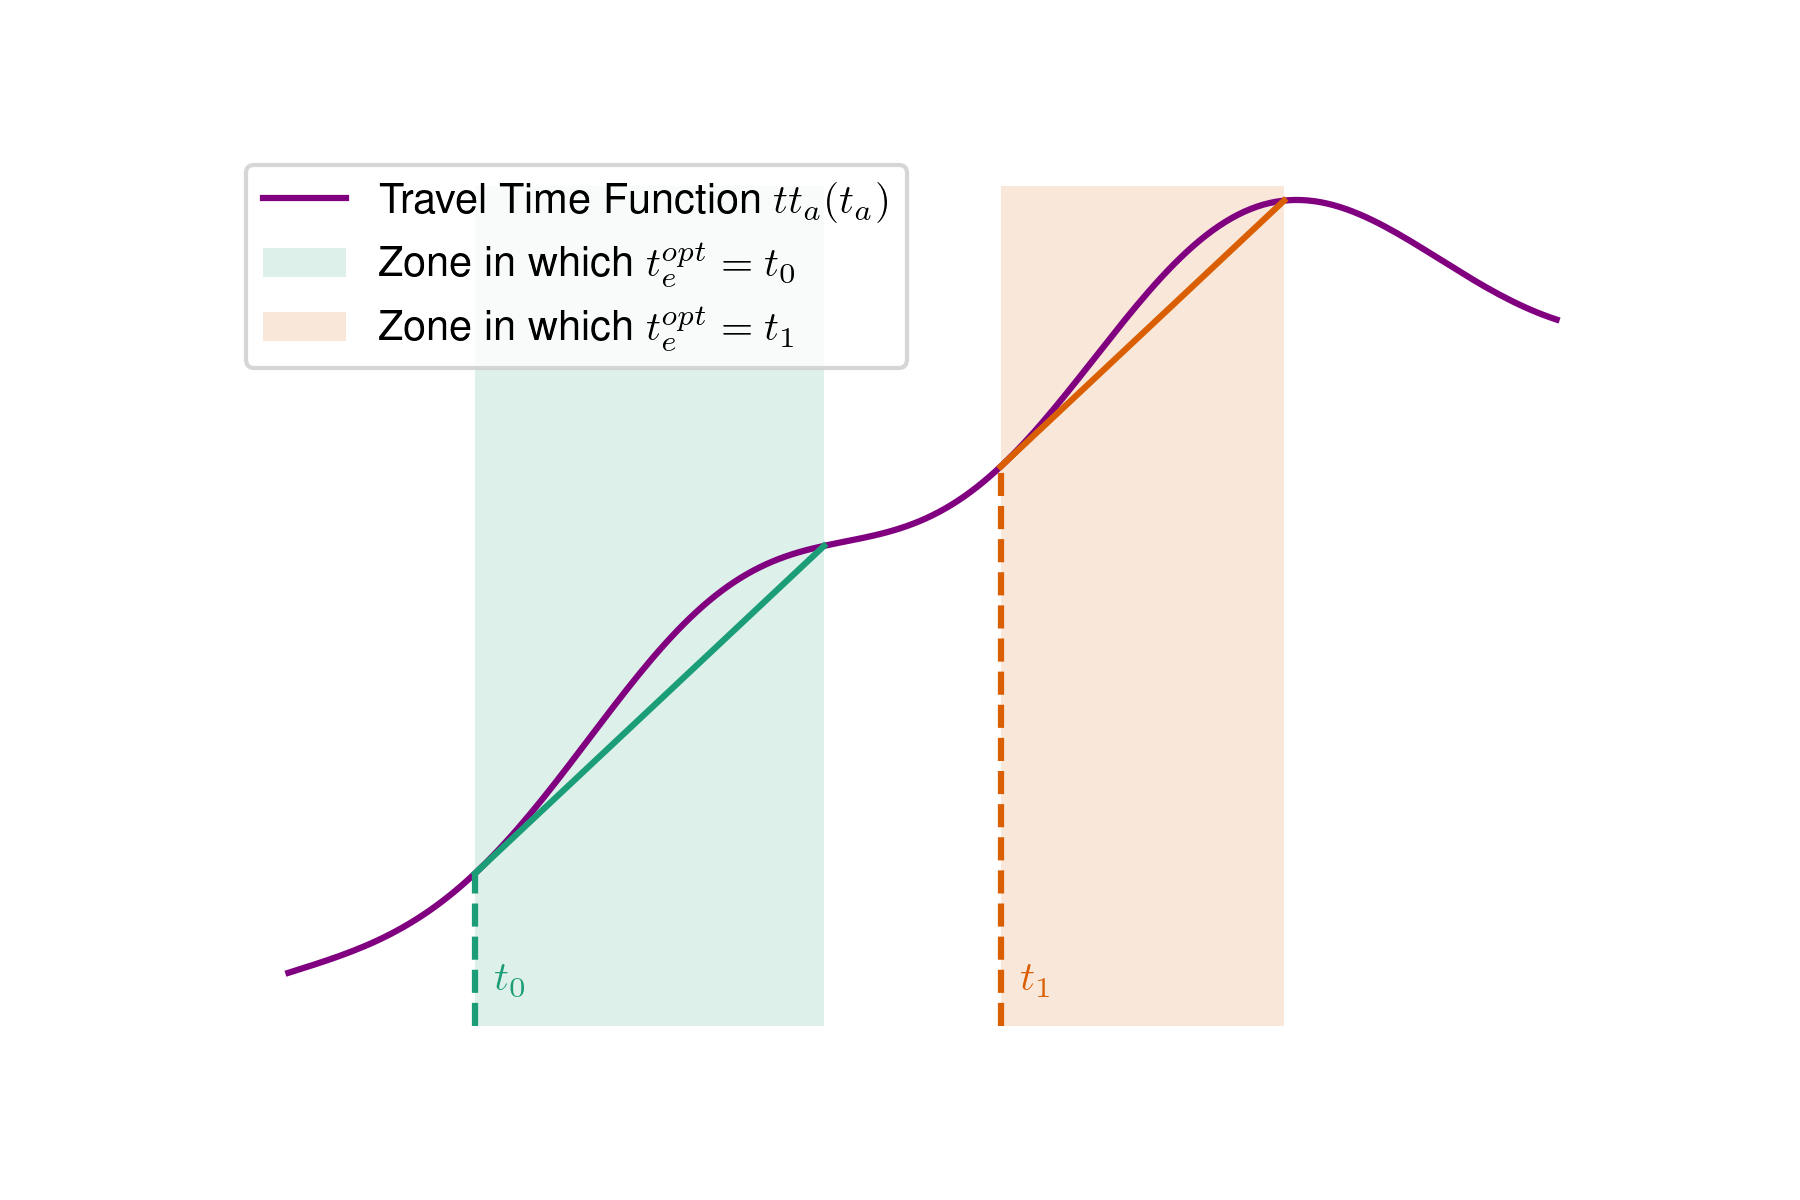
\includegraphics[width=.8\textwidth]{early_arrivals_jump}
  \caption{How the optimal early arrival changes,
    when changing the parameter \(t^*\).
    When \(t^*\) is in one of the shaded zones,
    the optimal early arrival time \(t_e^{opt}\) will be constant and equal to the time that yielded the zone.
  Otherwise, the optimal early arrival does not exist.}
  \label{fig:early_arrivals_jump}
\end{figure}

Figure~\ref{fig:early_arrivals_jump} shows this behaviour:
when \(t^*\) falls in the shaded zones,
the optimal early arrival \(t_e^{opt}\) is constant (in each of the zones).
If \(t^*\) is not in the zones,
the optimal early arrival is not defined:
for these values of the parameter,
the global minimum will be realized by either an on-time arrival (that is, \(t^{opt} = t^*\))
or by a late arrival.

The case of late arrival is, as expected, exactly symmetrical.

Once the dependency of the points \(t_e^{opt}, t_l^{opt}\) on the parameters has been explained,
the global minimum \(t^{opt}\) has to be characterized.
To this end, note that the optimum can only be smaller, greater or equal to \(t^*\):
\begin{obs}
  \label{obs:t_opt-dep}
  Given values for the parameters \(\beta, \gamma, t^*\) one out of the following is always true:
  \begin{itemize}
  \item \(t^{opt} = t_e^{opt}\) that is, the optimal arrival is an early arrival
  \item \(t^{opt} = t_l^{opt}\) that is, the optimal arrival is a late arrival
  \item \(t^{opt} = t^*\) that is, the optimal arrival is an on-time arrival
  \end{itemize}
\end{obs}

The following lemma gives a strong condition on when an on-time arrival can be realized:
\begin{lemma}
  \label{lemma:where-no-ot}
  If the parameters \(\beta, \gamma, t^*\) are given such that the optimal arrival time is an on-time arrival, that is
  \begin{equation*}
    t^{opt} = t^*
  \end{equation*}
  then the optimal early arrival \(t_e^{opt}\) and the optimal late arrival \(t_l^{opt}\) don't exist.
\end{lemma}
\begin{proof}
  Suppose thus the global minimum is realized in the point \(t = t^*\).
  
  By continuity of the cost function,
  early or late arrivals that realize a cost arbitrarily close to the global optimum can be found,
  by choosing them in a sufficiently small neighbourhood of the point \(t^*\).
\end{proof}

While the characterization of the points \(t_e^{opt}, t_l^{opt}\) was done in the proposition above,
describing the interaction between early and late arrivals is in general not easy,
and can be made simpler by assuming the travel time function to have some realistic features.

\begin{definition}
  \label{def:gen-tt-fun}
  Consider a function
  \begin{equation*}
    tt_a: \R \rightarrow \R
  \end{equation*}

  \(tt_a\) is said a \textbf{general travel time function} if it satisfies the following\todo{Put this as assumptions}:
  \begin{enumerate}
  \item \(tt_a \in C^1(\R)\)\todo{Add limits to \(\pm\infty\). Adapt later, where it says \textit{first requirement} etc}
  \item \(tt_a'(t_a) < 1\ \forall\, t_a\in \R\)
  \item \(tt_a\) is unimodal
  \end{enumerate}
\end{definition}

The first requirement is not restrictive,
since the space \(C^1(\R)\) is dense in the space of continuous functions,
and the travel time function can be assumed to be continuous.
Requirement about the bounded derivative arises from Lemma~\ref{lemma:bounded-der-tt}.
Unimodality, finally, is a restrictive requirement that has never been mentioned earlier,
and simplifies the problem of describing the interactions of early and late arrivals.
It is anyway realistic:
if considering only one out of the morning and evening peak (that can be treated separately),
we indeed expect the traffic pattern to be unimodal\todo{Cite something}.

Under these assumptions, when a set of parameters results in an early or late arrival can be clearly stated:
it is indeed possible to find a point before which the arrivals can only be either early or on-time,
and after which the arrivals can only be late or on-time:

\begin{figure}
  \centering
  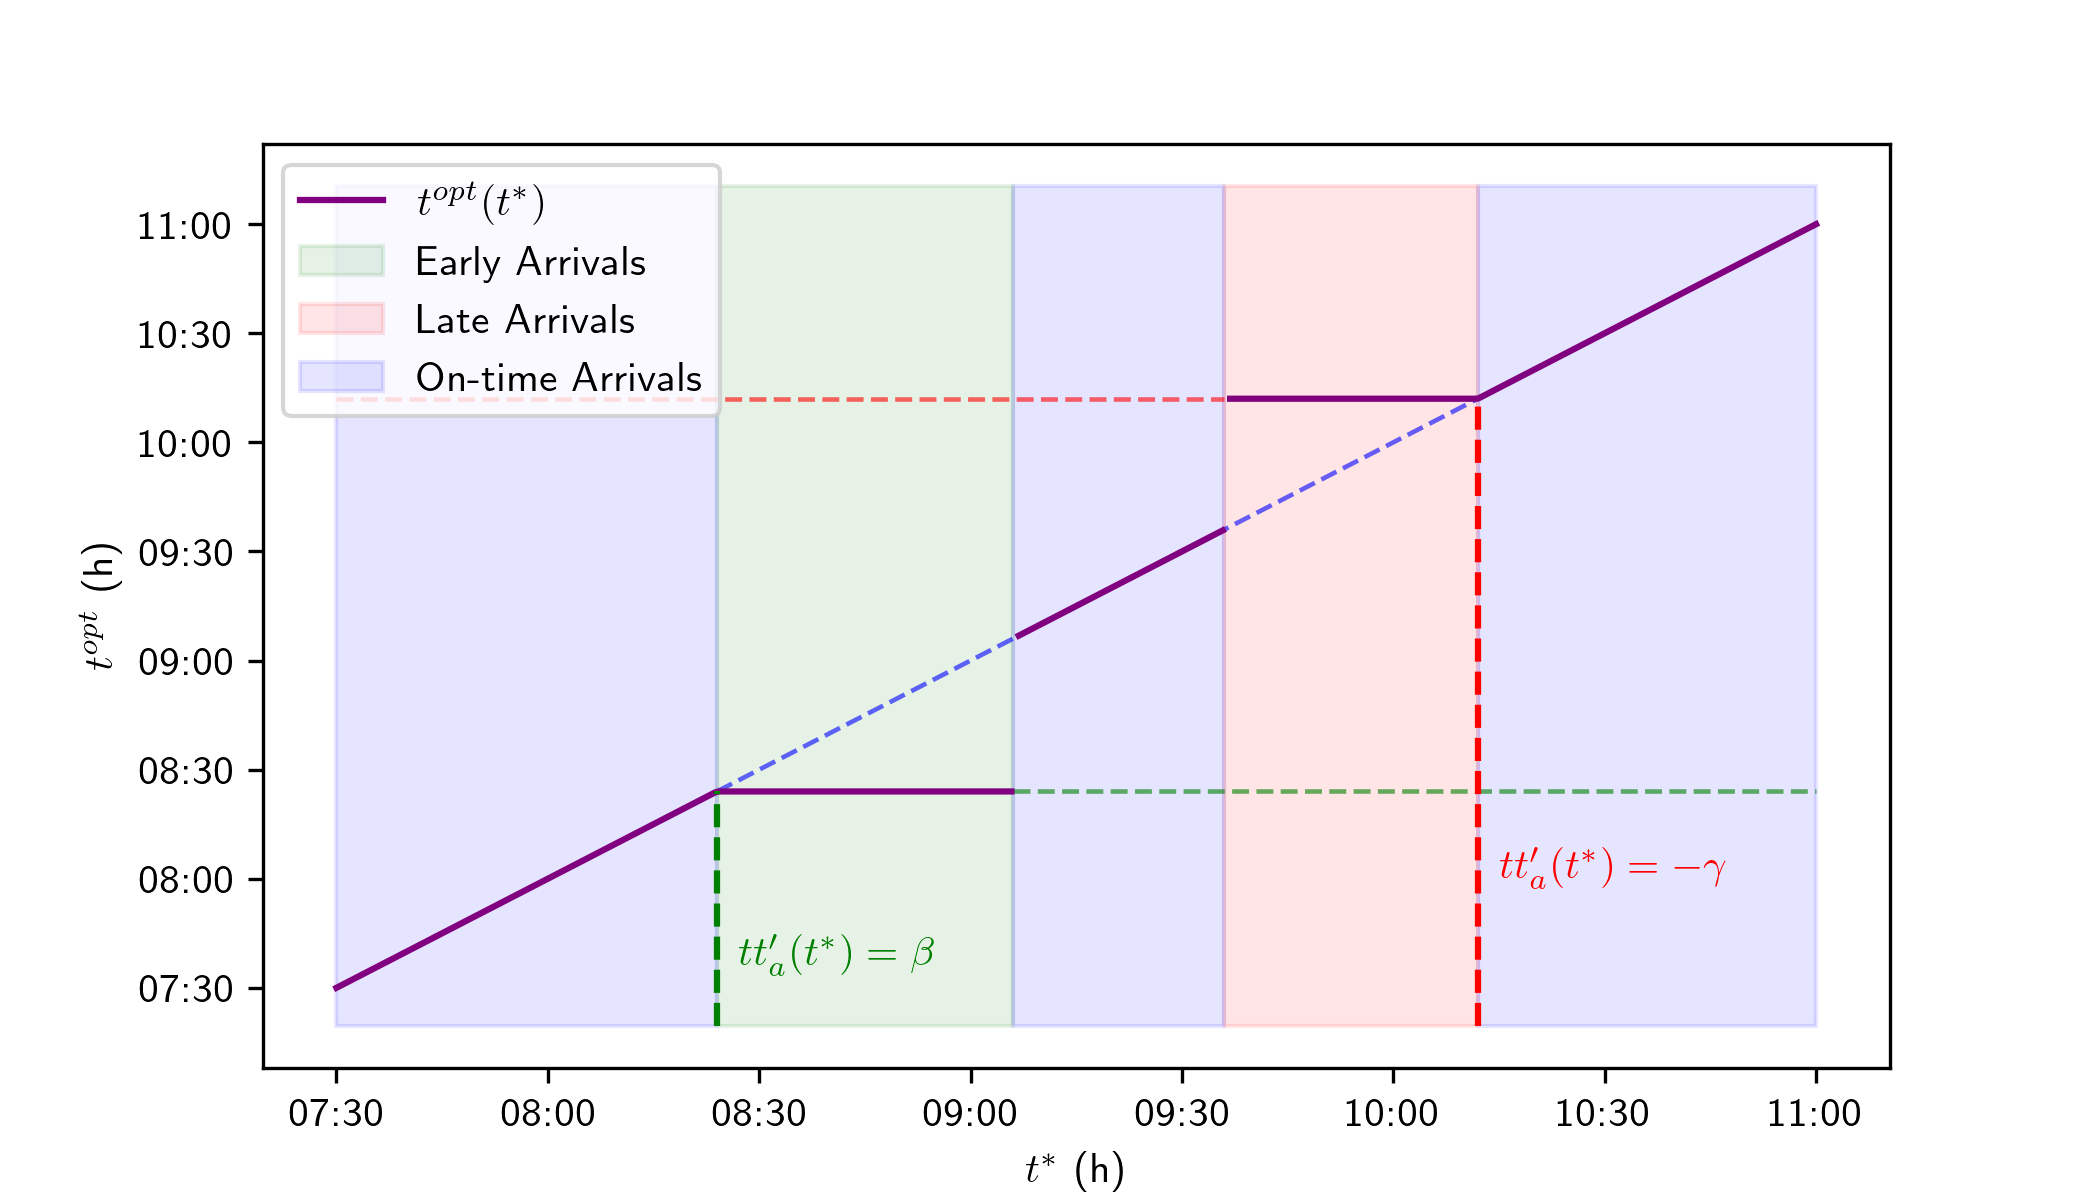
\includegraphics[width=.8\textwidth]{monotone_t_a}
  \caption{c}
  \label{fig:monotone-t_a}
\end{figure}

\begin{prop}
  \label{prop:split-early-late}
  \textcolor{red}{We need unimodality}
  Let \(tt_a\) be a general travel time function, the parameters \(\beta, \gamma\) be given.
  There exists a critical arrival time \(t_s(\beta, \gamma) \in \bar{\R} = \{\R \cup \pm \infty\}\) that satisfies
  \begin{itemize}
  \item If \(t^* < t_s(\beta, \gamma)\), then no late arrivals are observed:
    \begin{equation*}
      t^{opt}(\beta, \gamma, t^*) \neq t_l^{opt}(\beta, \gamma, t^*)
    \end{equation*}
  \item If \(t^* > t_s(\beta, \gamma)\), then no early arrivals are observed:
    \begin{equation*}
      t^{opt}(\beta, \gamma, t^*) \neq t_e^{opt}(\beta, \gamma, t^*)
    \end{equation*}
  \end{itemize}

  Moreover, when \(t^* = t_s(\beta, \gamma)\) arriving early or late yields the same cost:
  \begin{equation*}
    C(t_e^{opt}(\beta, \gamma, t_s); \beta, \gamma, t_s) = C(t_l^{opt}(\beta, \gamma, t_s); \beta, \gamma, t_s)
  \end{equation*}
\end{prop}
\begin{proof}
  
  
  % To prove the first part of the proposition,
  % it is enough to show that if 
  If there is no point realizing a late arrival, that is\footnote{For the scope of this proposition, how the parameters \(\beta, \gamma\) change is not relevant:
  for notational simplicity, the dependency of the points \(t^{opt}, t_e^{opt}, t_l^{opt}\) on these parameters are thus hidden,
  and the only dependency to be explicitly denoted will be the one on the desired arrival time \(t^*\).}
  \begin{equation*}
    \nexists\, t^* |\, t^{opt}(t^*) = t_l^{opt}(t^*)
  \end{equation*}
  then the proposition is true, for \(t_s = \infty\).

  Otherwise, consider a point \(t_0\) realizing a late arrival:
  \begin{equation*}
    t^{opt}(t_0) = t_l^{opt}(t_0)
  \end{equation*}

  We will now prove that a desired arrival time later than \(t_0\) cannot yield an early arrival:
  in the following, is shown that, given \(t_1 > t_0\),
  \begin{equation*}
    t^{opt}(t_1) \neq t_e^{opt}(t_0)
  \end{equation*}

  The proof will be divided in two different cases:
  \(t_1\) can be either greater or smaller than \(t_l^{opt}(t_0)\).

  At first, we suppose it to be smaller: \[t_1 \leq t_l^{opt}(t_0)\]

  This case will be again divided in two different cases:
  \(t_e^{opt}(t_1)\) can be either greater than \(t_0\) or smaller.

  Suppose now the second case:
  \begin{equation*}
    t_e^{opt}(t_1) \leq t_0
  \end{equation*}
  In this case, arrival at \(t_l^{opt}(t_0)\) is a realizable late arrival when the desired arrival time is \(t_1\) as well.
  Its cost will be lower than the cost of the same arrival,
  when the desired arrival time is \(t_0\):
  this is because the cost decreases on the distance between the desired arrival time (in this case, \(t_1\)) and the actual arrival time (in this case, \(t_l^{opt}(t_0)\)).
  \begin{align*}
    C(t_l^{opt}(t_0); \beta, \gamma, t_1) & = tt_a(t_l^{opt}(t_0)) + \gamma(t_l^{opt}(t_0) - t_1) \\
                                          & < tt_a(t_l^{opt}(t_0)) + \gamma(t_l^{opt}(t_0) - t_0) \\
                                          & = C(t_l^{opt}(t_0); \beta, \gamma, t_0)
  \end{align*}
  Moreover, the cost of every possible early arrival increases:
  the arrival time \(t_e^{opt}(t_1)\) is, on top of this, a realizable early arrival even when the desired arrival time is \(t_0\),
  and its cost is lower in this case:
  similarly, to the earlier computations,
  \begin{align*}
    C(t_e^{opt}(t_1); \beta, \gamma, t_1) & = tt_a(t_e^{opt}(t_1)) + \beta(t_1 - t_e^{opt}(t_1)) \\
                                          & > tt_a(t_e^{opt}(t_1)) + \beta(t_0 - t_e^{opt}(t_1)) \\
                                          & = C(t_e^{opt}(t_1); \beta, \gamma, t_0)
  \end{align*}
  There exists thus, when the desired arrival time is \(t_0\),
  a late arrival whose cost is lower than the one of the best early arrival:
  \begin{align*}
    C(t_l^{opt}(t_0); \beta, \gamma, t_1) & < C(t_l^{opt}(t_0); \beta, \gamma, t_0) \\
                                          & < C(t_e^{opt}(t_1); \beta, \gamma, t_0) \\
                                          & < C(t_e^{opt}(t_1); \beta, \gamma, t_1)
  \end{align*}

  Consider now the case in which the optimal early arrival is greater than the desired arrival \(t_0\):
  \begin{equation*}
    t_e^{opt}(t_1) > t_0
  \end{equation*}

  In this case, the travel time function has to be increasing at \(t_e^{opt}(t_1)\),
  being it an early arrival (as shown in Observation~\ref{obs:foc}),
  and by unimodality it has to be increasing at \(t_0\) as well.
  The cost of a late arrival at \(t_l^{opt}(t_0)\) is, on the other hand, decreasing:
  \begin{equation}
    \label{eq:cost-comp-1}
    \begin{split}
      C(t_l^{opt}(t_0); \beta, \gamma, t_1) & = tt_a(t_l^{opt}(t_0)) + \gamma(t_l^{opt}(t_0) - t_1) \\
                                            & < tt_a(t_l^{opt}(t_0)) + \gamma(t_l^{opt}(t_0) - t_0) \\
                                            & = C(t_l^{opt}(t_0); \beta, \gamma, t_0)
    \end{split}
  \end{equation}

  Moreover, the optimality of \(t_l^{opt}(t_0)\), when the desired arrival time is \(t_0\), yields
  \begin{equation}
    \label{eq:cost-comp-2}
    \begin{split}
      C(t_l^{opt}(t_0); \beta, \gamma, t_0) & < C(t_0; \beta, \gamma, t_0) \\
                                            & = tt_a(t_0)
    \end{split}
  \end{equation}

  Suppose now \(t_e^{opt}(t_1) > t_0\).

  Being the function \(tt_a\) increasing, its value in \(t_e^{opt}(t_1)\) will be greater than at \(t_0\):
  \begin{equation}
    \label{eq:decreasing-tt_a}
    tt_a(t_0) \leq tt_a(t_e^{opt}(t_1))
  \end{equation}

  Finally, the cost of an arrival at \(t_e^{opt}(t_1)\) will be lower bounded by the travel time:
  \begin{equation}
    \label{eq:cost-low-bound}
    \begin{split}
      C(t_e^{opt}(t_1); \beta, \gamma, t_1) & = tt_a(t_e^{opt}(t_1)) + \beta(t_1 - t_e^{opt}(t_1)) \\
                                            & > tt_a(t_e^{opt}(t_1))
    \end{split}
  \end{equation}

  By using equations \eqref{eq:cost-comp-1}, \eqref{eq:cost-comp-2}, \eqref{eq:decreasing-tt_a} and \eqref{eq:cost-low-bound},
  we get
  \begin{align*}
    C(t_e^{opt}(t_1); \beta, \gamma, t_1) & > tt_a(t_e^{opt}(t_1)) \\
                                          & \geq tt_a(t_0) \\
                                          & > C(t_l^{opt}; \beta, \gamma, t_0) \\
                                          & > C(t_l^{opt}(t_0); \beta, \gamma, t_1)
  \end{align*}
  showing that there is a late arrival whose cost is smaller than the best early arrival for \(t_1\).


  Consider, finally, the case in which \[t_1 > t_l^{opt}(t_0)\]

  Note that the reasoning above shows, given the arbitrariness of the choice of \(t_1\),
  \begin{align*}
    C(t_e^{opt}(t_1); \beta, \gamma, t_1) & > C(t_l^{opt}(t_0); \beta, \gamma, t_l^{opt}(t_0)) \\
                                          & = tt_a(t_l^{opt}(t_0))
  \end{align*}
  where, in the last line, the cost has been computed.

  Note now that the function \(tt_a\) has to be decreasing (again, given Observation~\ref{obs:foc}) at \(t_l^{opt}(t_0)\) and,
  as a consequence of unimodality,
  will be so until \(t_1\). This implies
  \begin{equation*}
    tt_a(t_1) \leq tt_a(t_l^{opt}(t_0))
  \end{equation*}

  The value of the travel time is a lower bound for the optimal cost,
  being it the cost of an on-time arrival.
  An early arrival will thus not be realized,
  since the cost for an on-time arrival will be lower:
  \begin{align*}
    C(t_1; \beta, \gamma, t_1) & = tt_a(t_1) \\
                               & \leq tt_a(t_l^{opt}(t_0)) \\
                               & = C(t_l^{opt}(t_0); \beta, \gamma, t_l^{opt}(t_0)) \\
                               & < C(t_e^{opt}(t_1); \beta, \gamma, t_1)
  \end{align*}

  This shows that \(t_1\) cannot yield an early arrival,
  if the function \(tt_a\) is decreasing at \(t_0\).

  This reasoning shows that, given a desired arrival time that realizes a late arrival,
  a greater desired arrival time will never yield an early arrival.

  A symmetric reasoning will show the same for early arrivals:
  given a desired arrival time that yields an early arrival,
  no earlier desired arrival times will yield late arrivals.

  These two statements prove the first part of the proposition:
  let indeed
  \begin{align*}
    t_{s, l} & = \inf\{t^* |\, t^{opt}(t^*) = t_l^{opt}(t^*)\} \\
    t_{s, e} & = \sup\{t^* |\, t^{opt}(t^*) = t_e^{opt}(t^*)\}
  \end{align*}

  Any choice of \(t_s \in [t_{s, e}, t_{s, l}]\) will satisfy the two requirements for \(t_s\).

  Regarding the second part of the proposition,
  that is, that the cost of arriving early or late at \(t_s\) is the same,
  it simply follows from a careful choice of the value \(t_s\).

  Note indeed that the cost of arriving early continuously grows as the value of \(t_s\) is increased from \(t_{s, e}\),
  while the cost of arriving late continuously grows as \(t_s\) is decreased from \(t_{s, l}\).

  Since the cost of arriving late when desiring \(t_{s, e}\) is greater than the cost of arriving early,
  and the cost of arriving early when desiring \(t_{s, l}\) is greater than the cost of arriving late,
  there has to be a value for \(t_s\) that satisfies the claim.\todo{Better argue this}
\end{proof}

This proposition is the last result of the section,
as, if considered together with Proposition~\ref{prop:into-early-late} and Lemma~\ref{lemma:where-no-ot},
it completely characterizes the function \(t^{opt}(\beta, \gamma, t^*\).

It indeed defines a critical point,
dependant on the value of the parameters \(\beta, \gamma\),
that splits the domain of the function (in the dimension in which lies \(t^*\))
into two separate zones.

Into the two zones, Proposition~\ref{prop:into-early-late} can be used to compute the exact minimum:
Once the intervals where the optimal early (or late) arrival is defined,
Lemma~\ref{lemma:where-no-ot} can be applied to precisely characterize the type of arrival that is realized for the given values of the parameters and,
eventually, at what time the arrival occurs.

This will be at the core of the method used in the next section:
in a slightly simpler setting, the arrival time \(t_s\) will be computed,
as well as the points \(t_e, \bar{t_e}, t_l, \bar{t_l}\).
The value of the parameter \(t^*\) will then be compared to these points

%%% Local Variables:
%%% mode: LaTeX
%%% TeX-master: "../main"
%%% End:
